\section{Virtual Meeting Place}
\label{sec:virtualMeetingPlace}
\label{sec:projectgroup}
In this section we analyze the requirement Virtual Meeting Place.
Related requirements are: Navigate to Project Groups and Project Group Members.
These are analyzed in \secref{sub:designprojectgroupnavigation} and \secref{sub:projGrpMembers}.
%The following is an analysis of the requirement Virtual Meeting Place.

A virtual meeting place can take many forms.
As our requirement of a virtual meeting place states, we want it to comply with the Aalborg PBL model.
We analyze our requirements based on the conducted interviews and demo meetings and our own experiences.

We refer to the tools that our peer-groups develop as \detdeandrelaver{}s.
The aspects of the requirement Virtual Meeting Place that are presented here are: Structure of virtual meeting place, assignment of virtual meeting place, division of projects and groups, and virtual project tools integration.
These are presented below.


\subsection{Structure of the Virtual Meeting Place}
The members of a project group should have a place where they can meet and engage in project work using related \detdeandrelaver[]s.
Recall from \secref{sec:subSysDef} that our responsibility is to construct a place where this can happen, not construct the actual \detdeandrelaver[]s.
We have to decide the structure of the virtual meeting place.
%The two structures considered are described below.
We consider two different approaches, which are described below.
\pagebreak{}

\paragraph{Shared Group} One idea is to have every project group share everything with other project groups in a semester.
This corresponds to having every project group working in the same room in the real world.

\paragraph{Team Group} Another idea is to give a virtual group room to every project group and ensuring that only the members of the project group and the supervisors can contribute to the work on the project.
The corresponding situation in the real world is that every project group has their own group room where only they (and their supervisors) can do work on the project. \\

The Shared Group idea requires less effort than the Team Group idea to implement since no permissions need to be considered.
However, the Team Group is closer to the way that the Aalborg PBL model should work in practice.

We choose the Team Group structure. 
It is infeasible to have every project group share everything.
A project group member could be forced to look through a lot to find the relevant information to the given project group.
Furthermore, by allowing each project group to have their own virtual meeting place, the members can customize the place as they see fit by removing irrelevant tools and possibly adding new relevant tools.
The virtual place where these tools can be found is called the ``virtual group room''.
A virtual meeting place for a project group thereby consists of the virtual group room and the tools available.
This is illustrated on \figref{fig:projectgrouproom}.
\begin{figure}%
\center
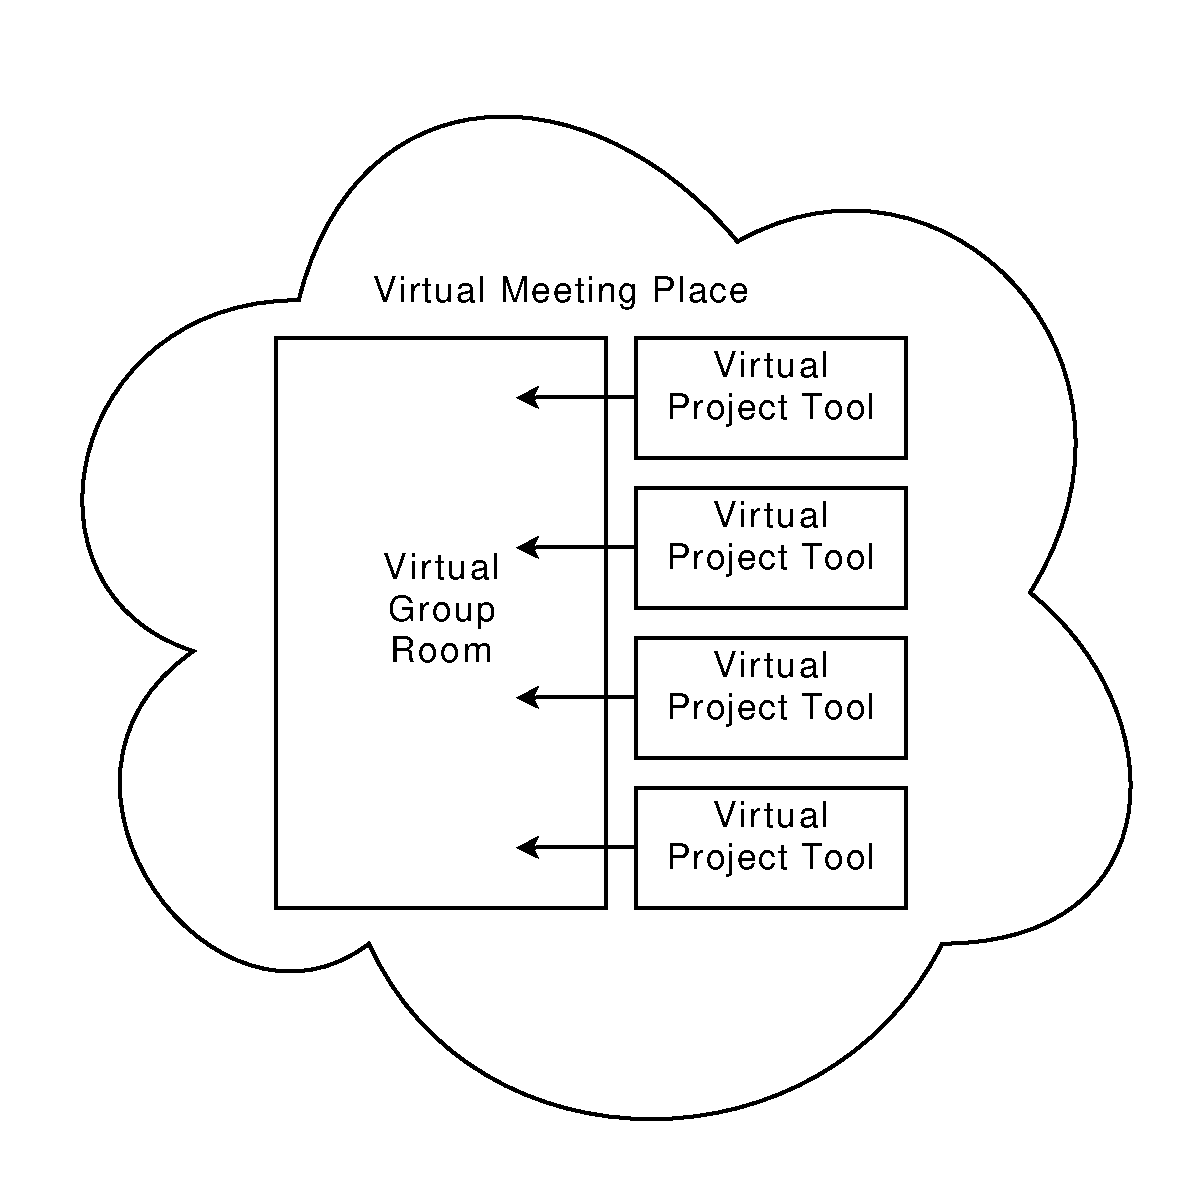
\includegraphics[scale=0.50]{images/VirtualMeetingPlace}%
\morscaption{The connection between the virtual meeting place and the virtual group room}%
\label{fig:projectgrouproom}%
\end{figure}
%For the rest of the report we refer to the virtual meeting place as the ``project group room''.

The virtual group room should have some of the same project related tools as a physical group room.
We as the \administrationgroup{} team implement the virtual group room, and the other three peer-groups implement the different tools.
%We as the \groupname{} implement the project group room, and the other three peer-groups implement the blocks (see \secref{subsec:blocks}) that provide different functionality.
%wrapper for the three other groups
%Joining of tools


\subsection{Assignment of Virtual Meeting Places}
At Aalborg University the physical group rooms are assigned to project groups periodically.
The period at which assignment of physical group rooms occur can differ.
Some of the most common periods are presented here:
\begin{itemize}
	\item \textbf{Never} There are no physical group rooms available because the field of study does not follow the Aalborg PBL model or the students are studying from remote locations.
	\item \textbf{Daily} The students have to reserve the physical group rooms on a daily basis (as stated in \appref{sec:jettePia}).
	\item \textbf{Half-yearly} Physical group rooms are assigned to each project group at the start of each semester.
\end{itemize} 

The virtual meeting place should be a hub where tools central to group work are available.
It should be similar to physical group rooms at Aalborg University in usage, and be available on a half-yearly basis.


\subsection{Division of Projects and Groups}
\label{sub:divProjGroup}
So far we have regarded project groups as an atomic entity, but projects and groups can be regarded as two different entities.
%In the Aalborg PBL model projects and teams exists as two different entities. 
The question arises if project groups should be designed as groups that have a relation to a project or as a single entity, where the group and project are one.
Below are the properties of the two variants presented.

%We will now list the properties of the two different variants. 

\paragraph{Groups and Projects Divided} 
\begin{itemize}
	%\item Projects and groups have a many-to-many relationship.
%	\item Directly reflects the objects of Aalborg PBL model. %Når jeg læser PBL Aalborg haløj ser jeg ikke hvorfor denne her passer bedst, der tager man jo udgangs punkt i et project/problem og dertil hører ét team, ikke flere teams.
	\item Flexibility between projects and groups, allowing many-to-many relationship.
	\item Complex to implement.
\end{itemize}


\paragraph{Groups and Projects United}
\begin{itemize}
	\item A group is linked to a single project; they are inseparable.
	\item Simple to implement.
\end{itemize}
%We will now examine related design options.

\begin{figure}[p]%
\centering
        \begin{subfigure}[b]{0.8\textwidth}
                \centering
                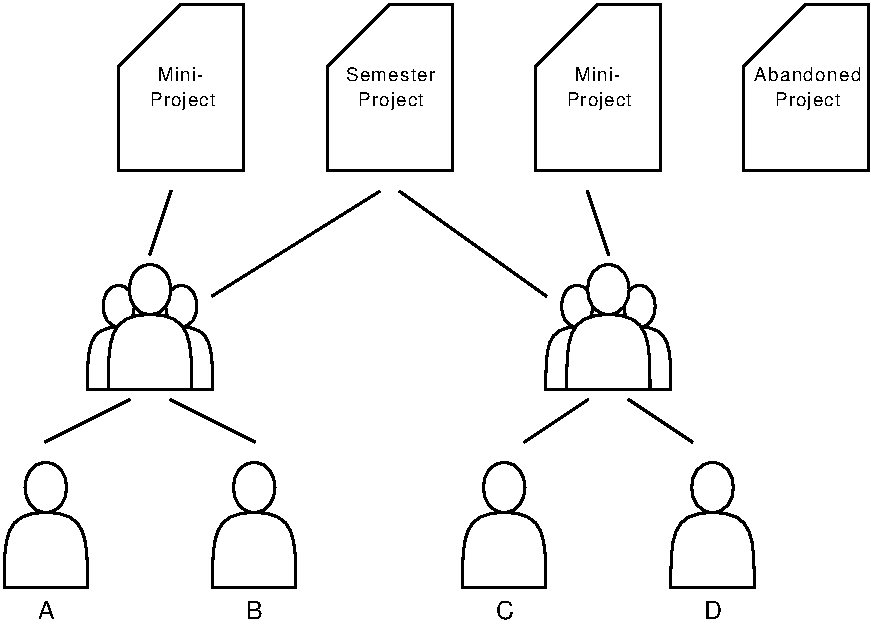
\includegraphics[width=\textwidth]{images/groupprojectdivision.pdf}
                \morscaption{Divided}
                \label{fig:divProjGroup:div}
        \end{subfigure}%
				\vspace{10mm}
        \begin{subfigure}[b]{0.8\textwidth}
                \centering
                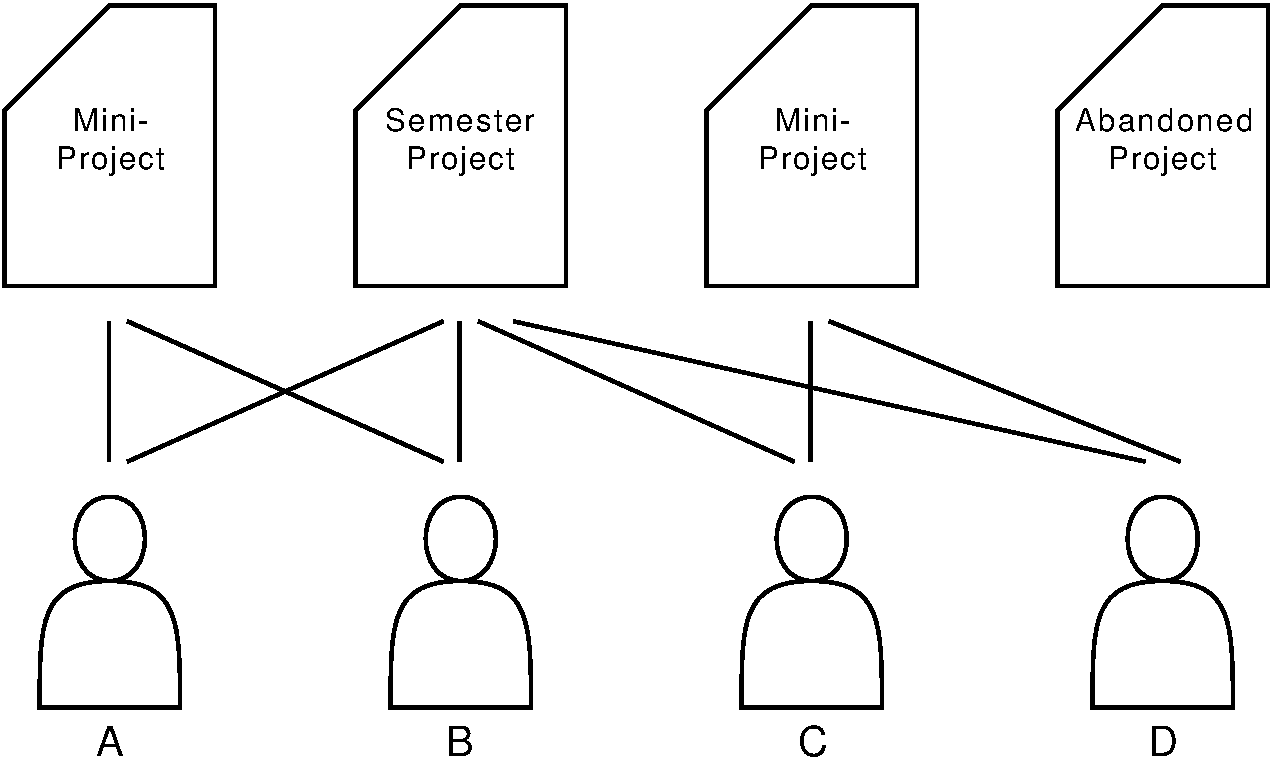
\includegraphics[width=\textwidth]{images/groupprojectunited.pdf}
                \morscaption{United}
                \label{fig:divProjGroup:united}
        \end{subfigure}%
\morscaption{The difference between the two approaches to the division of project and group illustrated by an example}%
\label{fig:divProjGroup}%
\end{figure}

The differences between these variants are illustrated with an example in \figref{fig:divProjGroup}.
The example is as follows:
There are four students identified by the letter A to D, and four projects; two mini projects, one semester project, and a single abandoned project.
Students A, B, C, and D collaborate on the semester project.
Students A and B are working on a mini project.
Students C and D are working on the other mini project.
Finally no one is working on the abandoned project.

Intuitively the option to divide groups and projects (seen in \figref{fig:divProjGroup:div}) might seem more appropriate since it introduces a level of indirection.
However, our interview with Lene (seen in \appref{sec:lene}) shows that the administrative personnel does not see any benefit from having any extra levels of indirection between students and projects.
%To select which of these divisions to choose we have contacted Lene W. Even and conducted an interview (seen in \appref{sec:lene}).
Since we are working agile we prefer to take the simplest viable approach and allow for extension of the system later.
We choose to design groups and projects as one entity (seen in \figref{fig:divProjGroup:united}) in accordance with the needs of our end users and to simplify our system.
The database design for storing project groups and members of the project group is found in \secref{sec:dbdesign}.
% -- note that we have not been in contacts with students for this decision.

\subsection{Virtual Project Tools Integration}
\label{sub:interActivities}
As mentioned previously we are developing a virtual group room where different \detdeandrelaver[]s can be used to perform project work.
The \detdeandrelaver[]s are primarily developed by our peer-groups.
For the \detdeandrelaver[]s to be available to the users through the virtual group room we have to have a common interface over which the virtual group room and the \detdeandrelaver[]s can communicate.
A typical communication message from the virtual group room to the \detdeandrelaver{} could be a request to make the tool render itself.
Alternatively we could integrate every tool directly into the virtual group room.
This, however, is not extensible enough.
Recall that we are four peer-groups of three to four students working together, which means that we would likely ``step on each others toes'' if we all were to work on the same component at the same time.
Furthermore, there is a group of students next year that must take over this project.
They might want to change the functionality or disable a tool.
This should be much easier if each tool is encapsulated in a component with a common interface than if every tool were intertwined in a single component.

Now that we have established that a there is a need for an interface between the \detdeandrelaver[]s and the virtual group room, we want to examine the possibilities that we have for doing so.
The two broad categories that the final choice can fall in are: Using an existing interface or developing a new interface.
These are not mutually exclusive.
We may take an existing interface and modify it to fit our needs.
Since we are making a plugin for an established LMS, we need to examine the possibilities in it to find an existing interface.
There are two plugin types in \moodle{} that we consider to be used as interface: \block{}s and activity modules.
Both of these are described in \secref{sub:plugins}.
By choosing any of these as the interface we restrict our peer-groups to make some or all of their \subsystem{} as the given plugin type, hence this is a joint decision.

%Intuitively the activity module might seem like the right choice, after all the name is \emph{activity} modules.
%However, activity modules are not for general \detdeandrelaver[]s, but only for course \detdeandrelaver[]s.
An activity module is required to have a database relation containing the instances of the activity module, each of which must have a link to a course~\cite{moodleactivitymodule}.
We do not use this idea because we do not want to have links between our project groups and courses -- a project group is an entity in its own right.

We now consider whether to use \block{}s or develop a new interface.
Developing a new interface would give us more freedom because we may choose exactly how it is defined.
On the other hand a \block{} ensures that \system{} will have a similar look and feel as the rest of \moodle{}.
Additionally, the students that take over next year will have accessible documentation through the \moodle{} Documentation about how to modify \detdeandrelaver[]s or add new ones.
The advantages of \block{}s outweigh the additional freedom that we may gain from defining our own interface.
This leads us to choose to use \block{} plugin type that every \detdeandrelaver{} must be implemented as.
For the virtual group room to communicate with \detdeandrelaver[]s it can use calls to member methods of \block{}s.
%E.g.\ to render a \block{} a call to \me{get\_content} is used~\cite{moodleblockapp}.
%\moodle{}, however, provides functionality to render all blocks associated with a given page.


\subsection{Navigation to Virtual Group Room}
\label{sub:designprojectgroupnavigation}
For a user to navigate to a virtual group room that he is a member of, there should be a procedure like the one for navigating to courses in which the user is enrolled.
To accomplish this we have looked at how navigation to courses work in \moodle{}.
There is currently a problem in Moodle when navigating to courses. 
When a user is enrolled in a large number of courses his entire front page is filled with links to those.
There is no built-in functionality to move or sort the links.
ELSA mentioned this problem during the meeting that we conducted with them described in \secref{sub:elsaInterview}.

We want to avoid this problem when we design the navigation for project groups.
Moodle has a navigation block with a list of important links.
We want to add an item to this list that, when expanded, shows the project groups the user is a member of.
Since a supervisor or an administrator might be a member of a many project groups, we want to limit the size of the list of project groups.
We do this by showing a maximum number of project groups according to a preset value.
If the user is a member of more project groups we show a link to a page that has a list of all the project groups that the user is a member of.


\subsection{Presentation of Members}
\label{sub:projGrpMembers}
Recall that the Presentation of Members requirement must ensure nearness for project group members.
If members of a project group tend to work in the same physical room, they have nearness.
To fulfill this requirement students conducting group work from remote sites should be able to experience nearness through our system.
The \supervisorgroup{} team has requested a feature for supervisors to see photographs of the members of a project group to help them identify a particular group.
We choose to design this feature to accommodate the requirement for project group members.
A part of the virtual group room should show all the members of the project group belonging to the room.
There should be a photography of the members to help identify them.
There is to be a functionality to hide or remove the members since students working in a physical group room might not need this and therefore prefer to focus on the other \detdeandrelaver[]s available in the virtual group room.

\subsection{Combining the Aspects}
In this section we combine the aspects discussed in the previous sections.
First and foremost there is a project group room where \detdeandrelaver[]s can be used directly or alternatively linked to.
Secondly there are all the \detdeandrelaver[]s that are not located directly in the virtual group room.
Only students and supervisor(s) associated with a project group are allowed to access the virtual group room of the given project group.
An exception to this is the administrative personnel, who have privileges to access and change any virtual group room.

Users are linked directly to project groups.
This reduces the complexity of the system at the cost of freedom.

Each \detdeandrelaver{} related to a virtual group room is implemented as a \block{}.
This allows for a well defined interface, which a virtual group room can use to communicate with the \detdeandrelaver[]s related to it.

To ensure familiar navigation for a user to his virtual group rooms, we extend the existing navigation menu of \moodle{}.
To avoid expanding the navigation menu out of proportions we limit the number of project groups that will be shown and provide an additional page where every project group belonging to a user can be found.

To provide a sense of nearness and to help supervisors recognize project groups, a simple tool is added to every virtual group room.
It can be hidden by users, if they do not need it.













\FloatBarrier